\documentclass[12pt,a4paper]{article}
\usepackage{graphicx}
\usepackage{csquotes}
\usepackage{centernot}
\usepackage{mathtools}
\usepackage{amsfonts}
\usepackage{algorithm}
\usepackage{amsthm}
\usepackage{caption}
\usepackage{array}
\usepackage{dsfont}
\usepackage{ amssymb }
\usepackage{blindtext}
\usepackage{hyperref}
\usepackage{amsmath}
\usepackage{breqn}
\usepackage{tikz}
\usepackage{pgfplots}
\renewcommand{\arraystretch}{1.3}
\usepackage[a4paper]{geometry}
\usepackage{multirow}
\usepackage{graphicx}
\usepackage[all]{xy}
\newtheorem{theorem}{Theorem}
\theoremstyle{definition}
\newtheorem{definition}{Definition}[section]
\theoremstyle{remark}
\newtheorem*{remark}{Remark}
\usepackage[noend]{algpseudocode}
\pgfmathdeclarefunction{poiss}{1}{%
	\pgfmathparse{(#1^x)*exp(-#1)/(x!)}%
}

\algrenewcommand\algorithmicrequire{\textbf{Input:}}
\newcommand\ddfrac[2]{\frac{\displaystyle #1}{\displaystyle #2}}
\newcommand\at[2]{\left.#1\right|_{#2}}
\usepackage{mathtools}
\DeclarePairedDelimiter{\ceil}{\lceil}{\rceil}
\graphicspath{ {images} }
%opening
\title{Bayesian Regression with COVID-19 spread data}
\author{Michele Guerrini, Davide Mozzi, Carlos Santillán}
\begin{document}
	\maketitle
	\begin{abstract}
		We present a Bayesian regression model for predicting the number of patients in a hospital and the ICU with COVID -19, given the number of patients in the same hospital and ICU, the number of new positive subjects and the region color of the previous week. 
	\end{abstract}
	
	\tableofcontents
	\newpage
	\section{Problem Description and Dataset}
	\subsection{Problem description}
	We are given the problem of predicting the number of patients in a hospital and the ICU 7 days from the current date. The prediction is based on the current date's patients both in the hospital and the ICU, new positive subjects, the average number of new positive subjects over the previous 7 days, and the color of the region. We tackle the problem via Bayesian regression
	\subsection{Dataset description}
	The dataset contains 205 entries. Each entry corresponds to a date with the following features
	\begin{enumerate}
		\item \textbf{newpos:} Number of newly detected COVID-19 positive subjects. An integer value.
		\item \textbf{intcar:} 	Number of COVID patients in the ICU. An integer value.
		\item \textbf{hosp:} Number of COVID patients at the hospital. An integer value.
		\item \textbf{newpos-av7D:} Average number of newly detected COVID-19 positive subjects over the previous 7 days. A float value.
		\item \textbf{color:} Color of the region over the previous 7 days. String that can contain the following values: \textit{Bianca}, \textit{Gialla}, \textit{Arancione}, \textit{Rossa}.
		\item \textbf{day:} Current date. String in R date format.
		\item \textbf{hospH8:} A target variable, the number of COVID patients at the hospital 7 days from now.
		\item \textbf{intcarH8:} A target variable, the number of COVID patients in the ICU 7 days from now.
		\item \textbf{dayH8:} The current date plus 7 days. 
	\end{enumerate}
	We will extend this by adding a categorical variable \textbf{season}, which will have values: \textit{winter}, \textit{spring}, \textit{summer}, \textit{fall}.
	\subsection{Data exploration}
	We start by looking at a pairs plot of the \textbf{newpos}, \textbf{intcar}, \textbf{hosp}, \textbf{newpos-avg7D}, and \textbf{hospH8}. The pairs plot contains a kernel density estimation of the distribution along the diagonal, the estimations are distinguished by color of the region. We also see the scatter plots for each pair of features, and the correlations between them for each region.
	\begin{figure}[htb!]
		\centering
		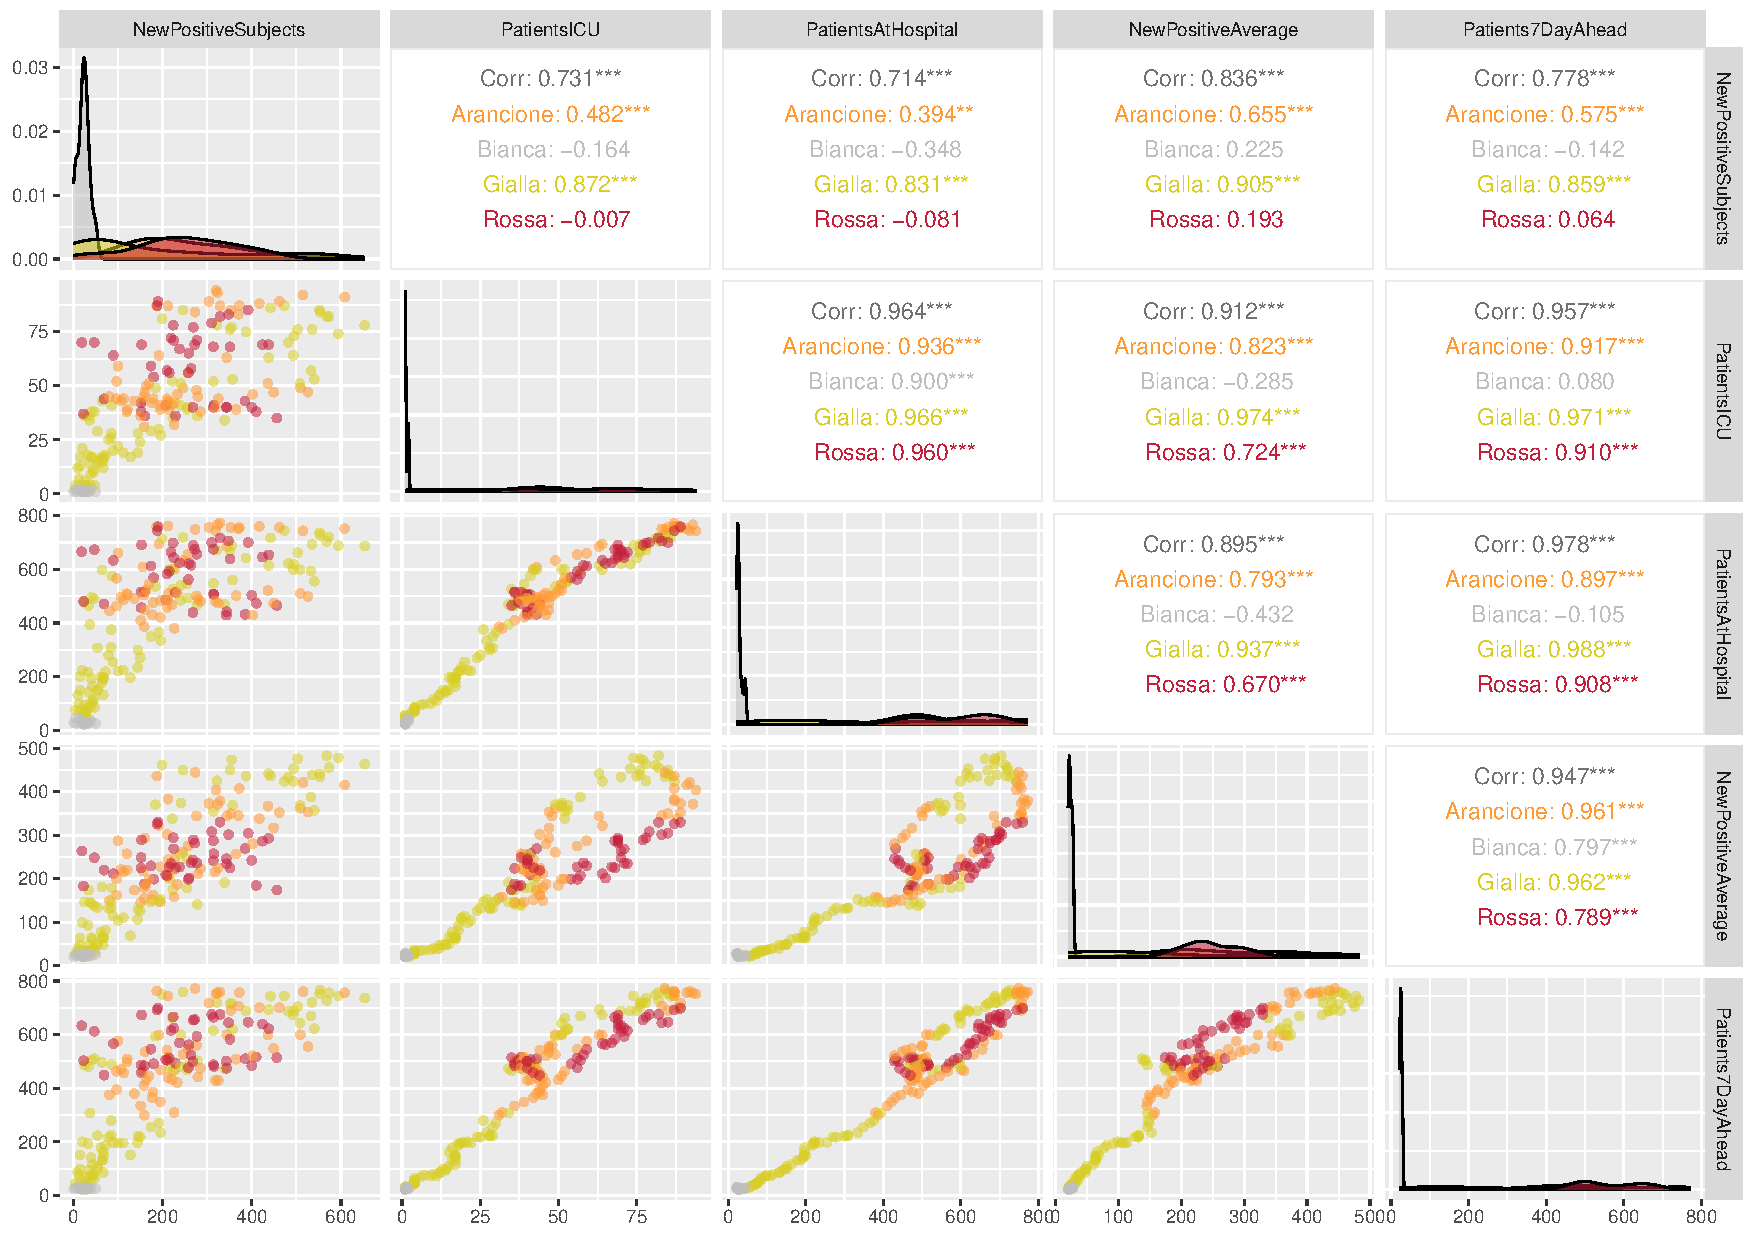
\includegraphics[width=150mm, height=115mm,scale=0.5]{corrplot.pdf}
			\caption{Pairs plot between the features and the number of patients at the hospital 7 days from now}
	\end{figure}
	
	
	We can immediately see an almost linear relationship between the number of patients in the ICU and those at the hospital, suggesting that we may remove one of them. The density plots are as we would expect, the white regions (lower COVID-19 presence) have all the mass concentrated around low values of the features, while the other regions are more spread out and have a center of mass further to the right (higher values). We also see that the relationship between the number of patients at the hospital, and that of 7 days in the future could be linear.
	
	\newpage
	We now look at the correlations with the number of patients in the ICU
		\begin{figure}[htb!]
		\centering
		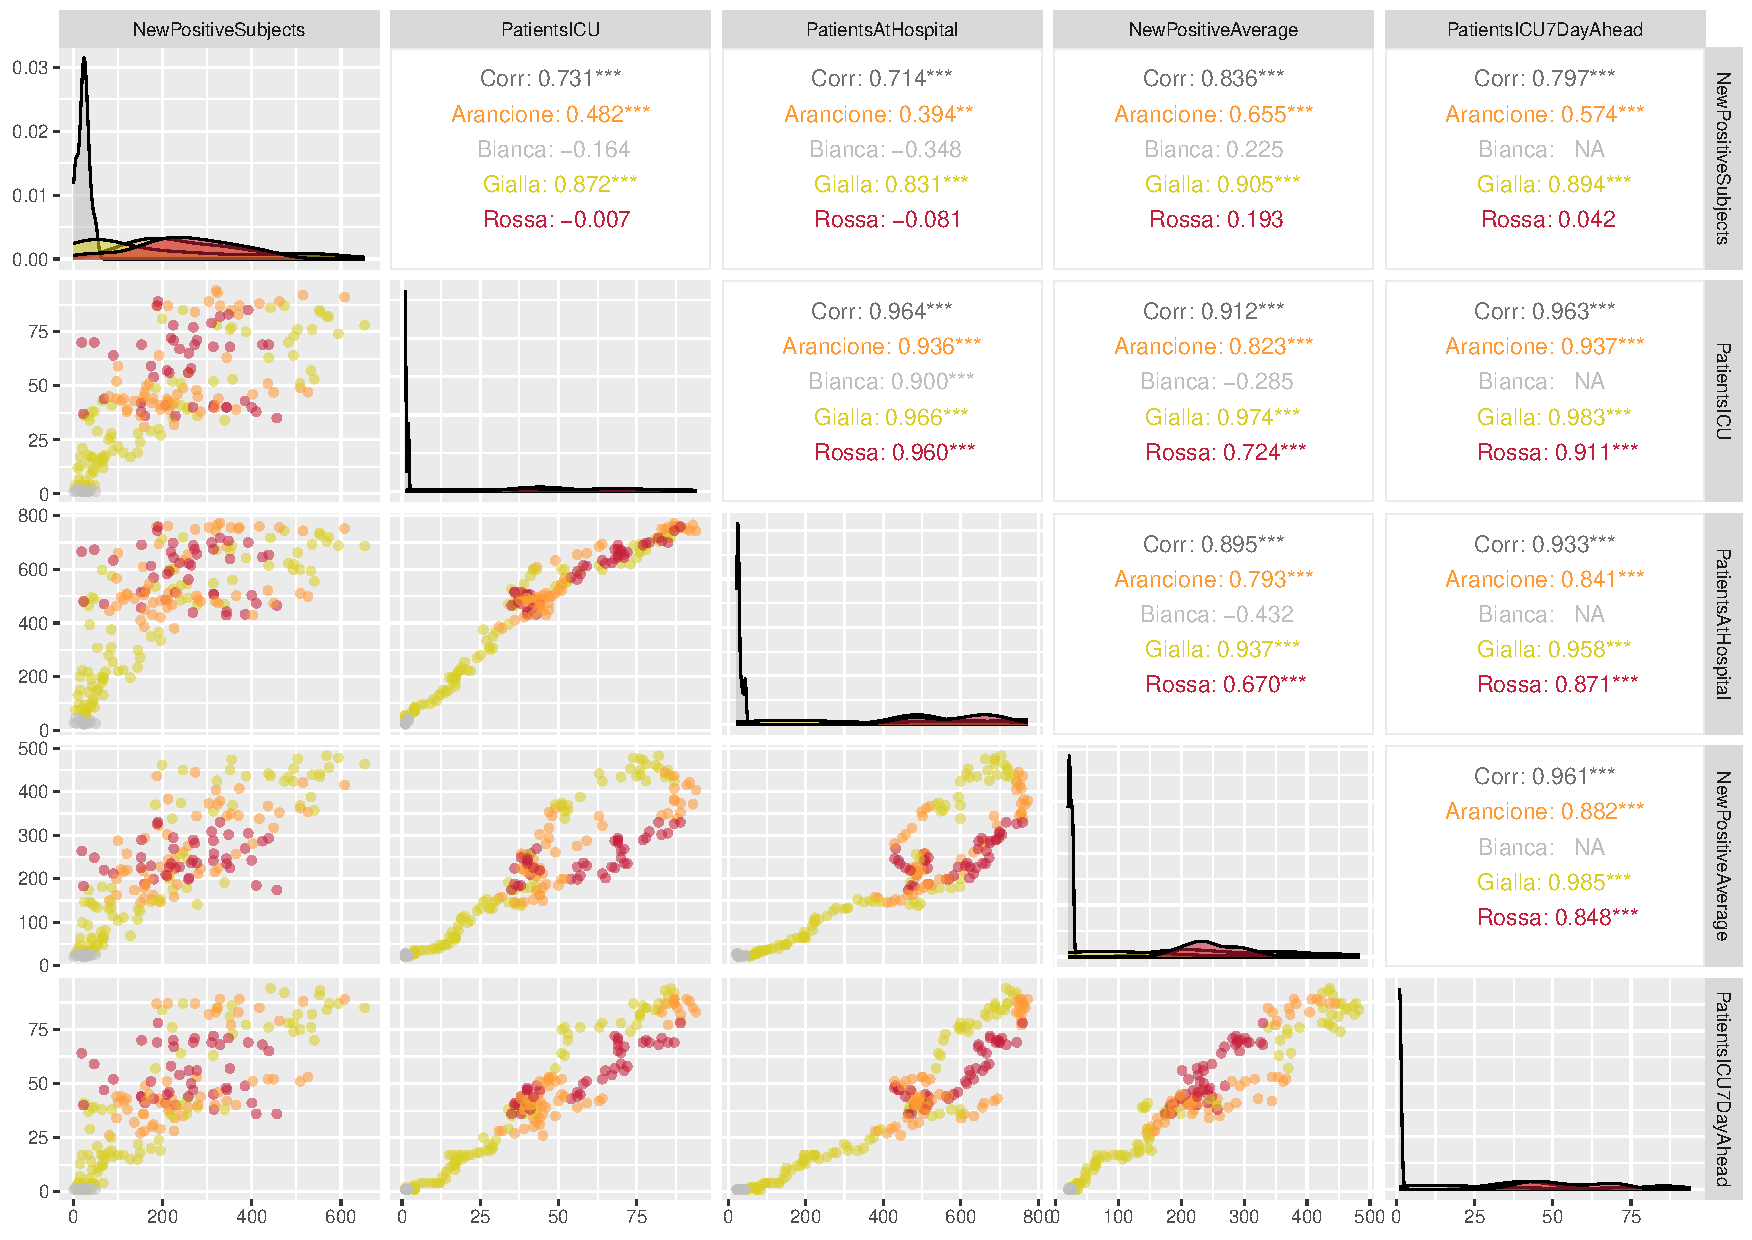
\includegraphics[width=150mm, height=115mm,scale=0.5]{corrplot1.pdf}
		\caption{Pairs plot between the features and the number of patients in the ICU 7 days from now}
	\end{figure}
	
	
	Again, for some of the features the relationship appears to be linear w.r.t. the target variable. Note that where the correlation is marked NA the value is zero. We used the Pearson correlation coefficient $r_{X,Y}$, defined as
	\begin{align*}
		r_{X,Y} = \frac{\sum(x_i-\overline{x})(y_i-\overline{y})}{\sqrt{\sum(x_i-\overline{x})^2\sum(y_i-\overline{y})^2}}
	\end{align*}


    Now we qualitatively assess how much each feature varies via boxplots (Figure 3). A boxplot allows us to see the spread of our data, the boxes themselves contain the interquantile range, the whiskers show the range of the rest of the data. We also mean center the features.
    	\begin{figure}[htb!]
    	\centering
    	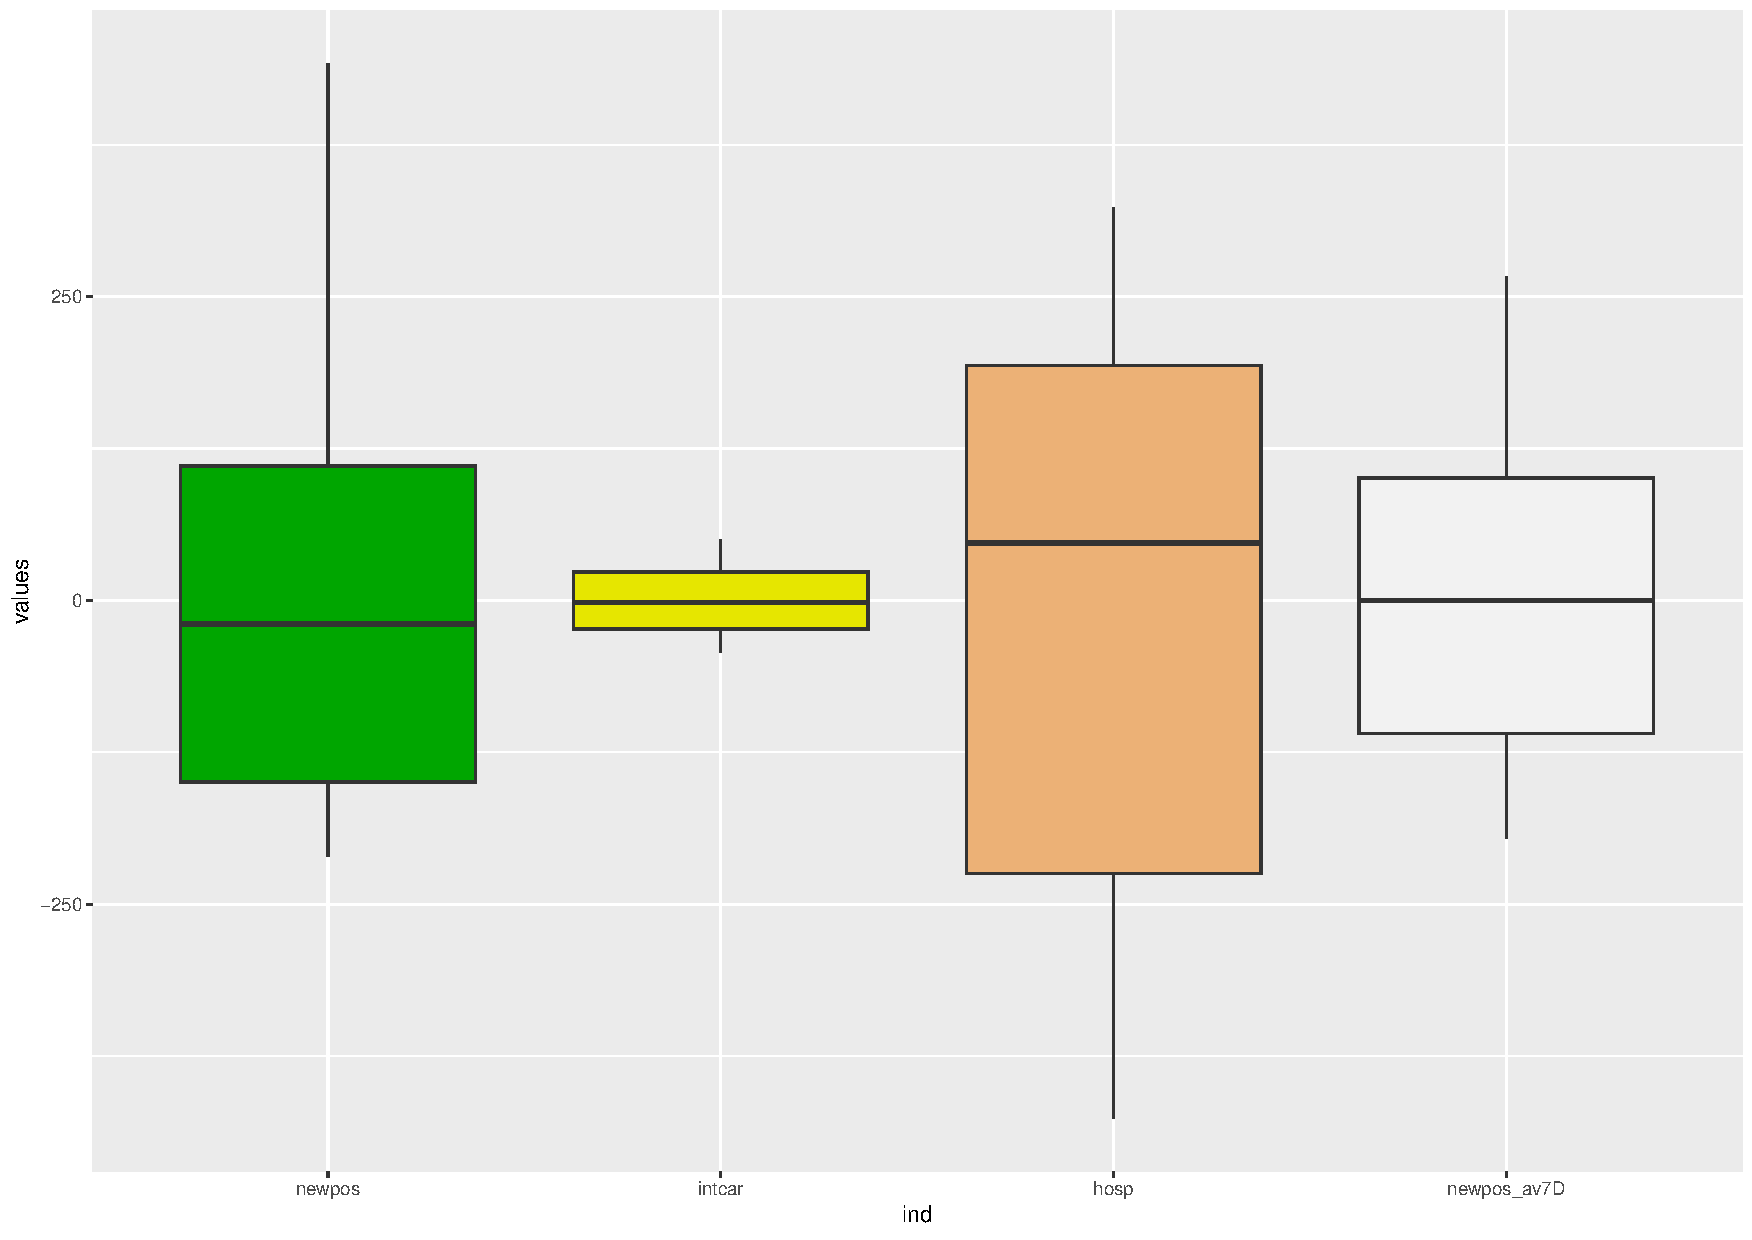
\includegraphics[width=100mm, height=80mm,scale=0.5]{box.pdf}
    	\caption{Boxplot of the mean-centered features}
    \end{figure}
    
    Since the some features vary greatly w.r.t. to others, see \textbf{intcar} and \textbf{hosp}, it could be a conventient to normalize the features.  In Figure 4 we see the boxplots for the normalized data.
    
    
     	\begin{figure}[htb!]
    	\centering
    	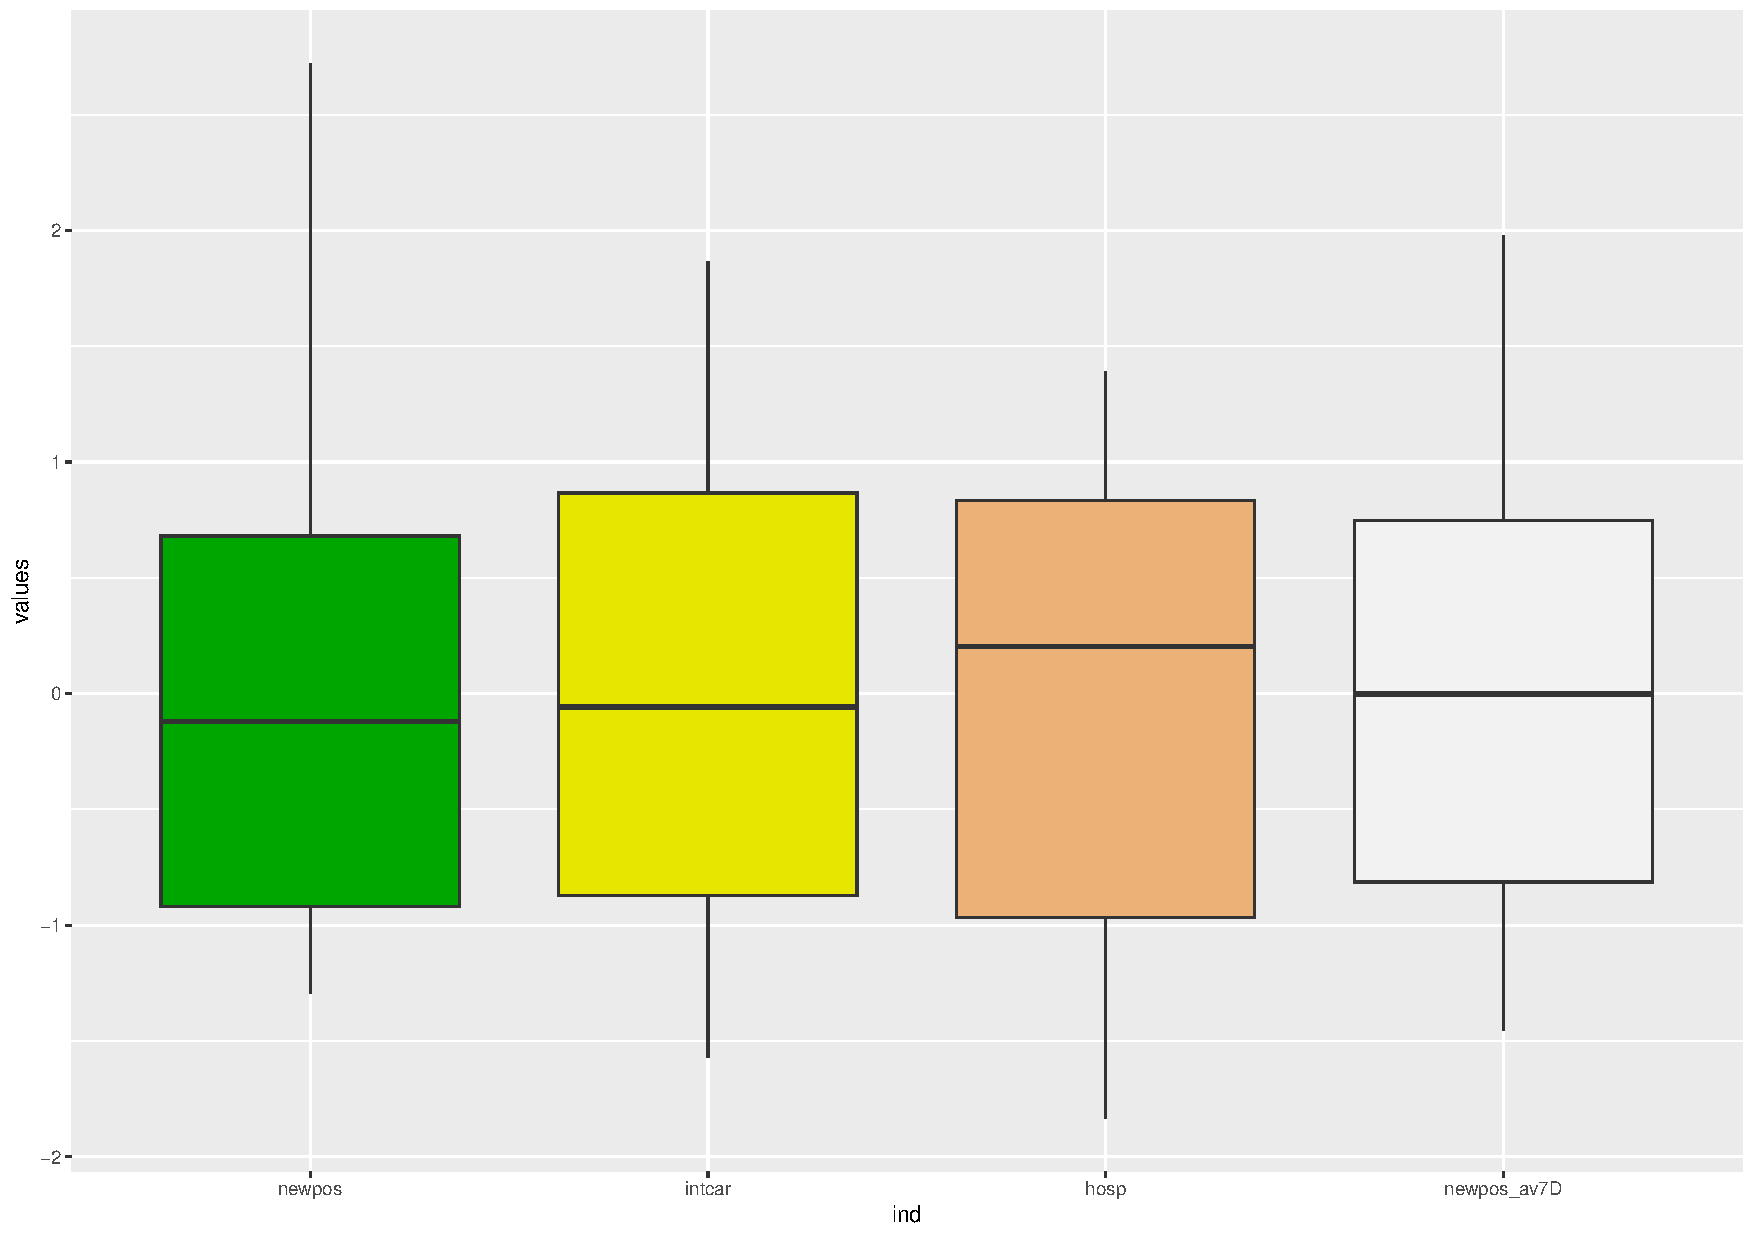
\includegraphics[width=100mm, height=80mm,scale=0.5]{boxplot2.pdf}
    	\caption{Boxplot of the mean-centered features}
    \end{figure}
    

Lastly, we take at the correlation matrices of the features. Figure 5 shows the full correlation matrix, no distinction made between regions. 

Figure 6 shows the correlation matrix for each region.
    
\begin{figure}[htb!]
	\centering
	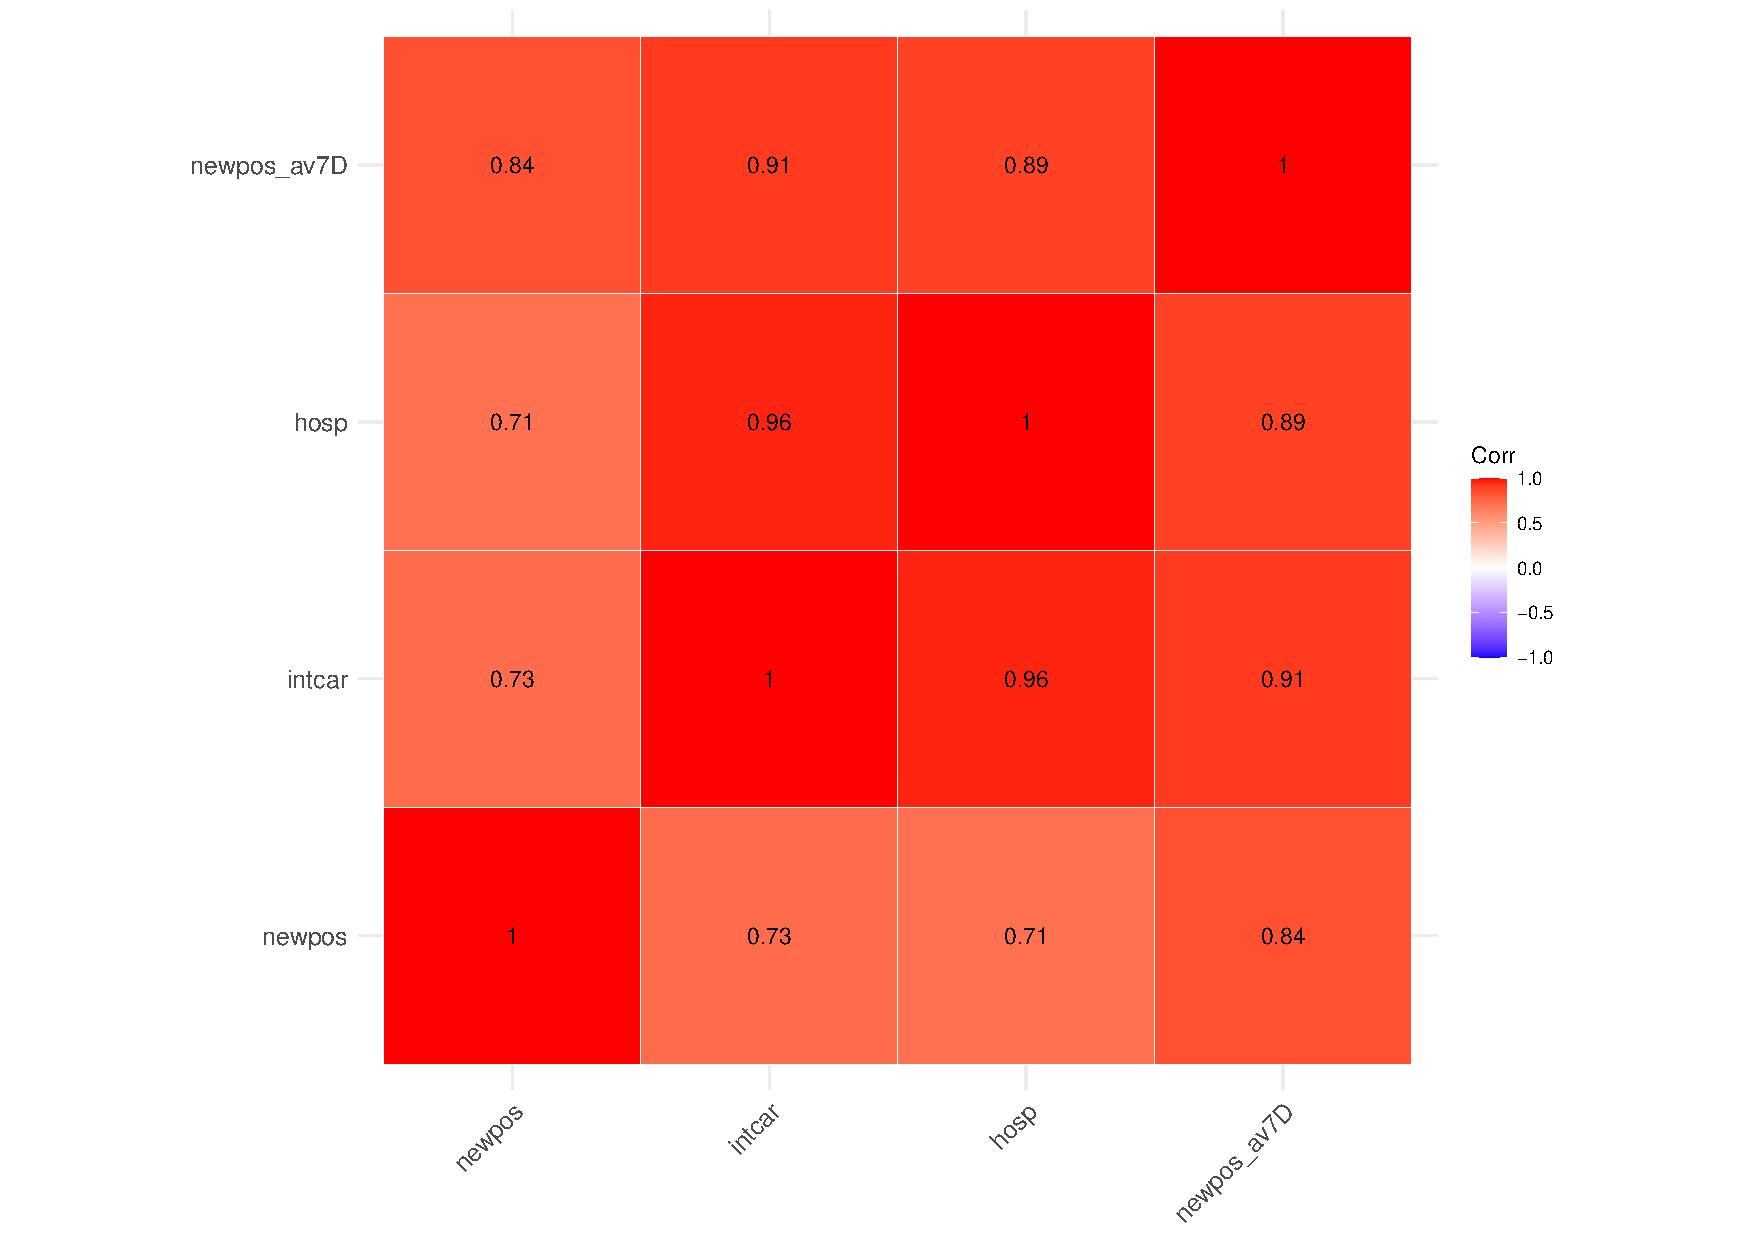
\includegraphics[width=75mm, height=60mm,scale=0.5]{corrmatrix.pdf}
	\caption{Correlation matrix of the features}
\end{figure}
\begin{figure}[htb!]
	\centering
	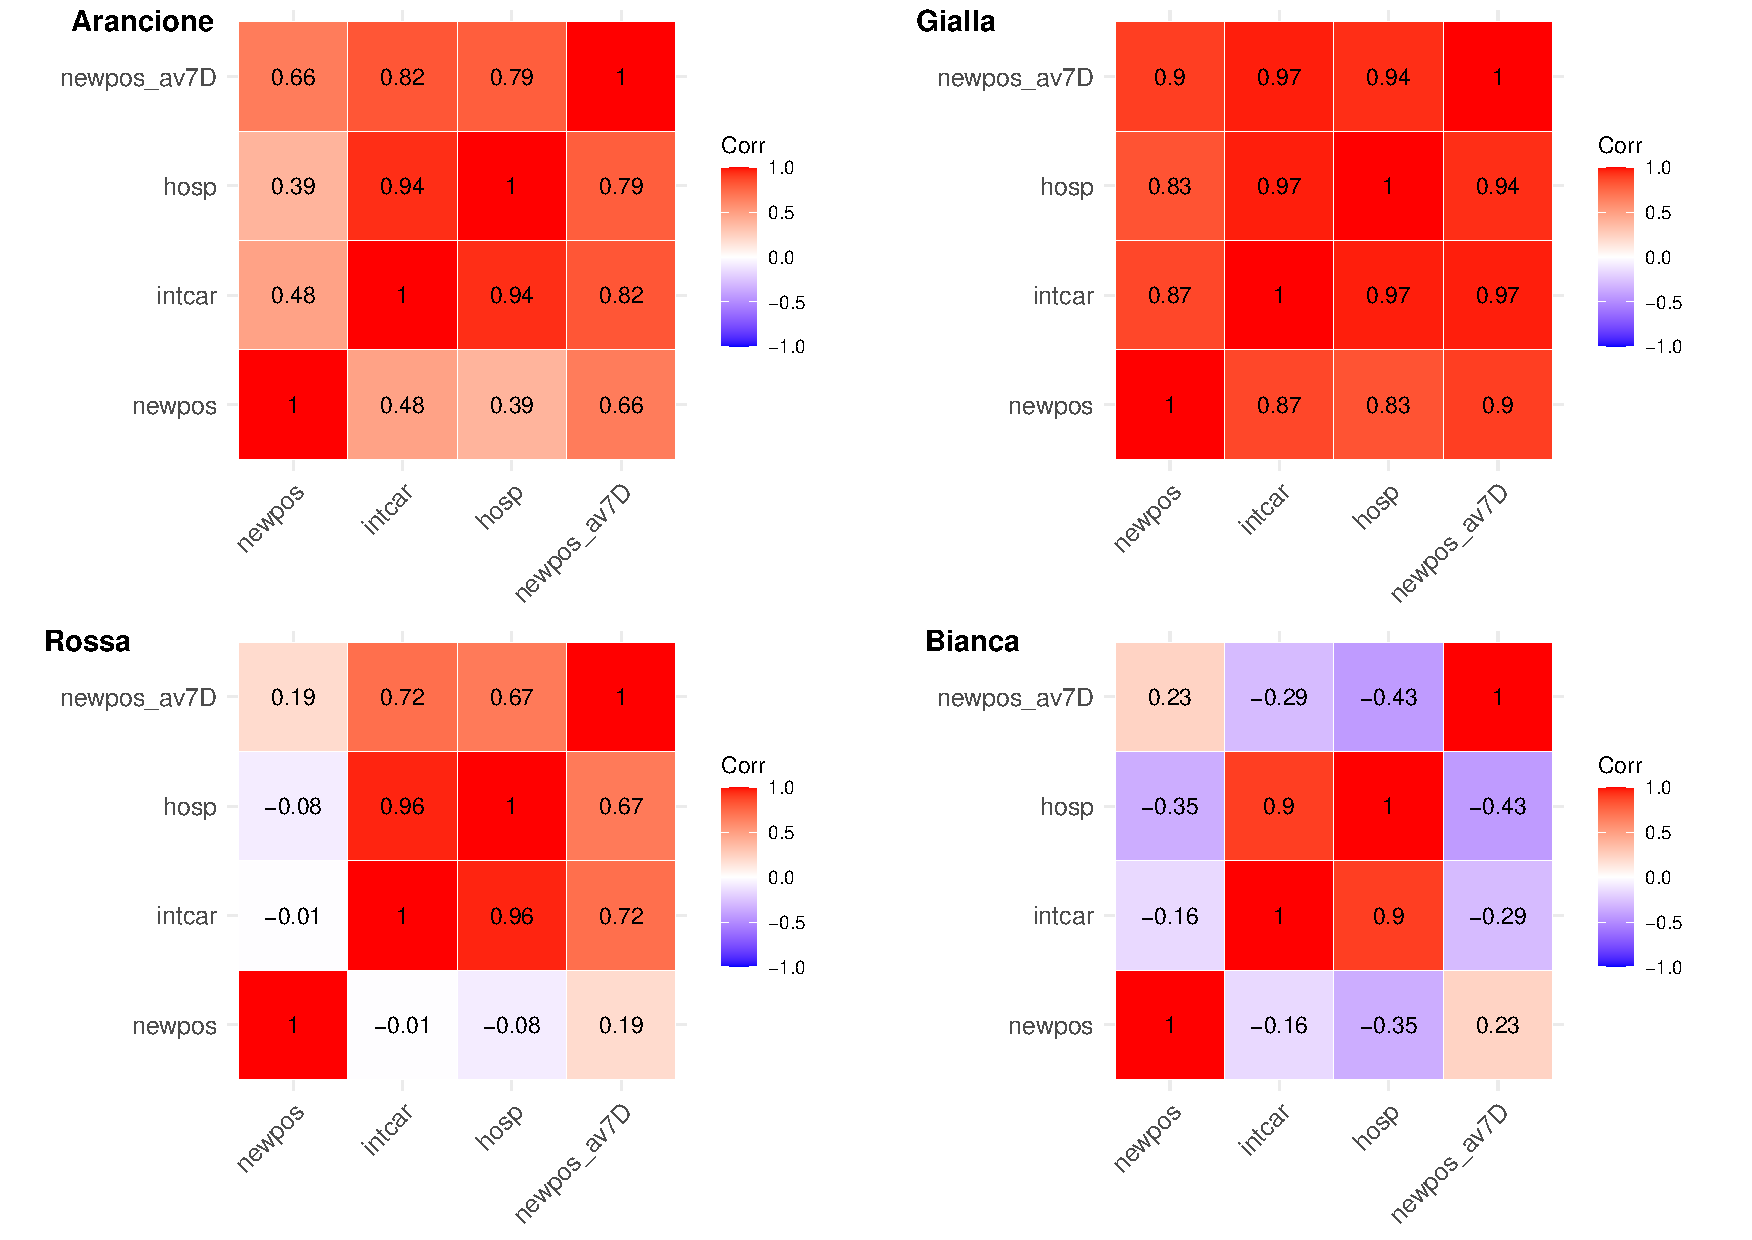
\includegraphics[width=130mm, height=100mm,scale=0.5]{corrmat2.pdf}
	\caption{Correlation matrix of the features per region}
\end{figure}
\end{document}